\subsection{Primeri big data arhitektur}

V tem odseku predstavimo nekaj arhitektur znanih podjetij~\cite{reference_architecture_classification_technologies}.
Na koncu predstavimo referenčno arhitekturo,
ki je povzeta iz članka~\cite{reference_architecture_classification_technologies} in je
podobna referenčni arhiteturi iz članka~\cite{reference_architecture_bd}.
Arhitektura Facebooka je predstavljena v sliki~\ref{fig:arch-facebook}, arhitektura Twitterja pa v sliki~\ref{fig:arch-twitter}.

\begin{figure}[H]
    \centering
    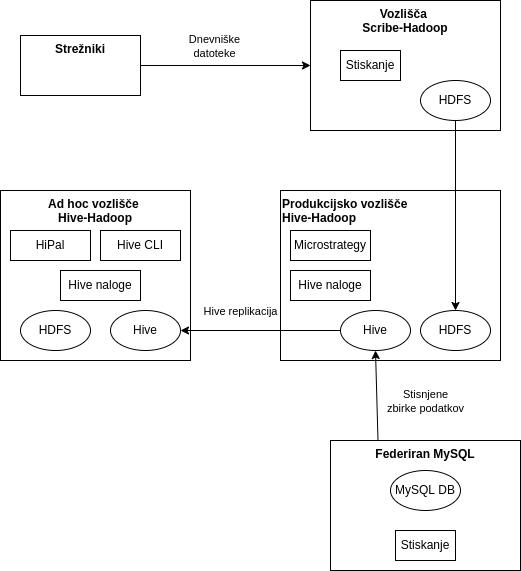
\includegraphics[width=0.6\textwidth]{images/arhitektura/podjetja/facebook.png}
    \caption{Arhitektura za analizo podatkov pri Facebook~\cite{reference_architecture_classification_technologies}.}
    \label{fig:arch-facebook}
\end{figure}

\begin{figure}[H]
    \centering
    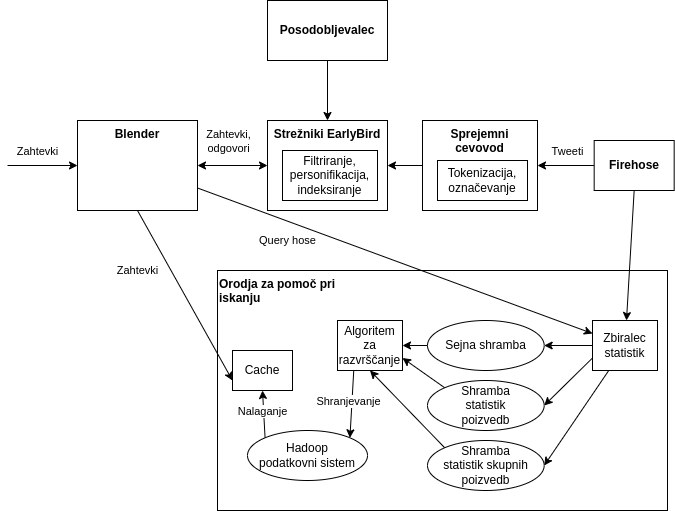
\includegraphics[width=0.8\textwidth]{images/arhitektura/podjetja/twitter.png}
    \caption{Arhitektura za analizo podatkov pri Twitterju~\cite{reference_architecture_classification_technologies}.}
    \label{fig:arch-twitter}
\end{figure}

\noindent Iz več primerov arhitektur, avtorji članka~\cite{reference_architecture_classification_technologies}
ustvarijo referenčno arhitekturo za Big Data, ki je predstavljena v sliki~\ref{fig:arch-ref-article}.

\begin{figure}[H]
    \centering
    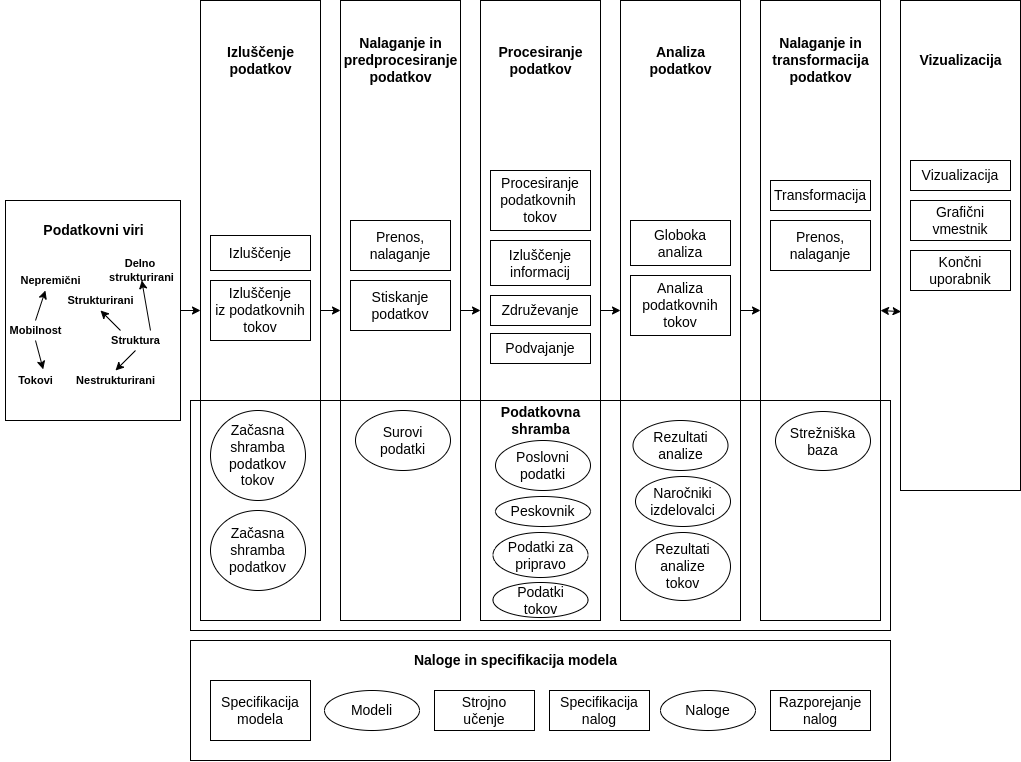
\includegraphics[width=0.99\textwidth]{images/arhitektura/reference.png}
    \caption{Visoko nivojska referenčna arhitektura Big Data aplikacij.
        Podatkovne shrambe so prikazane v elipsah, storitve v kvadratih in
        pot podatkov s puščicami.
        Povzeto po članku~\cite{reference_architecture_classification_technologies}.}
    \label{fig:arch-ref-article}
\end{figure}

\noindent V poglavju~\ref{sec:metodologija} referenčno arhitekturo uporabimo skupaj z
iteracijsko metodo~\cite{iterative_methodology} in
naredimo metodologijo.